%\documentclass[12pt]{article}
%\usepackage[latin1]{inputenc}
%\usepackage[spanish]{babel}
%\usepackage{latexsym}
%\usepackage{amssymb}
%\usepackage{amsmath}

%\setlength{\textwidth}{15cm}

%\newtheorem{ejem}{Ejemplo}
%\newtheorem{teor}{Teorema}
%\begin{document}
\chapter{DESARROLLO DEL PROYECTO}
El desarrollo del proyecto esta enfocado en dos ambientes, uno en el lado cliente, que se desarrollaron scripts para poder permitir la comunicación de los repositorios en GIT
el otro lado en el lado servidor para la elaboración del sistema web, que mantendrá informado a los desarrolladores
\section{METODOLOGIA DE DESARROLLO}
El desarrollo del proyecto 'Desarrollar un sistema Web microblog para notificación de acciones aplicadas en repositorios locales de desarrollo de proyectos de software versionados con GIT Esta basado en la metodología de desarrollo SCRUM.

\begin{figure}[htb]
\centering
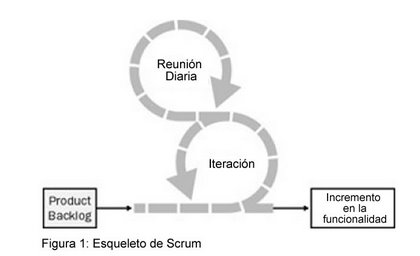
\includegraphics[width=0.7\textwidth]{imagenes/image-0.png}%ext=pdf,jpg,png
\caption{... texto ...}
\label{contexto:figura}
\end{figure}

Scrum es un proceso en el que se aplican de manera regular un conjunto de mejores prácticas para trabajar en equipo y obtener el mejor resultado posible de un proyecto. Estas prácticas se apoyan unas a otras y su selección tiene origen en un estudio de la manera de trabajar de equipos altamente productivos.

SCRUM es una metodología propuesta por los japoneses Hirotaka Takeuchi e Ikujijo Nonaka, un modo de desarrollo de carácter adaptable y orientada a las personas antes
que a los procesos, que controla de forma empírica y adaptable la evolución del proyecto con las siguientes prácticas de la gestión ágil:
       - Revisión de las iteraciones.
       - Desarrollo incremental, en el proyecto no se trabaja con diseño o
        abstracciones.
       - Desarrollo evolutivo, intenta predecir en las fases iniciales cómo será el
         resultado final y sobre dicha predicción realizar el diseño, la estructura del
        - producto no es realista, porque las circunstancias obligaran a remodelarlo
          muchas veces.
       - Auto-organización, los equipos son auto-organizados, con margen de decisión
         suficiente para tomar las decisiones que consideren oportunas.
       - Y colaboración entre todos según su conocimiento y no según su rol o puesto.

El resultado final en esta metodología se consigue de forma iterativa e incremental. Al comienzo de cada iteración (sprint) se determina qué partes se van a construir,
tomando como criterios la prioridad para el negocio, y la cantidad de trabajo que se podrá abordar durante la iteración. Dichas iteraciones se presentan en las etapas de
Especulación, Exploración y Revisión; y debido a que, según este tipo de modelos de desarrollo nunca se termina un producto, se presentan de forma infinita pudiendo
llegar a la etapa de cierre solo cuando se desee enviar al mercado una versión funcional del producto.

Reglas básicas
SCRUM tiene un conjunto de reglas muy pequeño y muy simple y está basado en los principios de inspección continua, adaptación, auto-gestión e innovación.
El cliente se entusiasma y se compromete con el proyecto dado que ve crecer el producto iteración a iteración y encuentra las herramientas para alinear el desarrollo
con los objetivos de negocio de su empresa.
Por otro lado, los desarrolladores encuentran un ámbito propicio para desarrollar sus capacidades profesionales y esto resulta en un incremento en la motivación de los
integrantes del equipo.
Ya hemos dicho que SCRUM es fácil y sencillo pero vamos a la materia, los siguientes son los elementos básicos de SCRUM:
    
    •   Una lista con las funcionalidades de la aplicación ordenadas de mayor a menor
        importancia. Esta lista se llama "Product Backlog". No hace falta que esta lista
        contenga todas las funcionalidades inicialmente.
    •   De la lista anterior, se toman las primeras funcionalidades, se descomponen en
        tareas y son anotadas en una lista que se llama "Sprint Backlog". Estas tareas
        serán realizadas en el siguiente mes.

Además de estos elementos tenemos unas cuantas reglas básicas y sencillas que
tenemos que cumplir:
    •   Una vez que se pasan las tareas más prioritarias del "Product Backlog" al
        "Sprint Backlog", estas no se pueden cambiar, esto quiere decir, que el trabajo
        de un mes queda fijado. Esta es la regla más importante de todas.
    •   Al final del mes, periodo denominado "Sprint", se tiene que tener un ejecutable
        con las funcionalidades del "Sprint Backlog".
    •   Todo el equipo puede añadir funcionalidades al "Product Backlog", pero sólo
        una persona puede ordenarlo. A esta persona se le denomina "Product
        Owner". Es el responsable del producto final.
    •   Cada día se hace una reunión de menos de 15 minutos, en la que se reúne
        todo el equipo: ingenieros y gestor (llamado "SCRUM Master") en la que cada
        miembro del equipo expone sólo los siguientes temas:
             o ¿Qué es lo que se hizo el día anterior?
             o ¿Qué es lo que se va a hacer hoy?
             o ¿Qué impedimentos tengo para realizar mi trabajo?


        Sólo se tratan estos temas para que la reunión sea rápida y no malgastar el
        tiempo de los demás. Si se tiene que tratar otro tema se hace otra reunión sólo
        con las personas implicadas. ¿Recordáis la serie de TV "Canción triste de Hill
        Street" en la que el sargento tenía una reunión matutina con sus agentes y que
        terminaba con un "Tengan cuidado ahí fuera"? pues viene a ser algo parecido.
    •   Al final del mes, es decir, al final del Sprint, se presenta el producto y se toman
        del "Product Backlog" las funcionalidades para cubrir en el siguiente mes.

La calidad en este caso, se logra y se mantiene de forma continua, pues se involucra
al cliente durante todo el tiempo que tarde el desarrollo, permitiéndole hacer aportes
que enriquezcan y generen nuevas funcionalidades y/o características al producto que
se está desarrollando.
Básicamente esto es todo.
Como se puede observar las reglas son sencillas, claras y es muy fácil de explicar y de
entender, lo que ayuda mucho a su implantación, pero no hay que engañarse, SCRUM
es un proceso de cambio, y uno además bastante serio.
SCRUM es sencillo, pero duro como una piedra, y se encuentra siempre mucha
resistencia:
    •   Los jefes de proyecto no querrán comenzar los proyectos sin tenerlo todo
        perfectamente identificado, acotado y planificado.
    •   Los desarrolladores no querrán la               responsabilidad    de  estimar   las
        funcionalidades y demostrar el producto.
    •   Los gerentes no querrán dejar tranquilo al equipo durante los Sprints.
    •   Etc.

\section{DESCRIPCION DEL PROBLEMA}

\section{PRUEBAS}
Durante las iteraciones en que se efectua el desarrollo de software segun la planificacion en la metodologia efectuada se realizaron las siguientes pruebas, estas siendo muy importantes ya que nos permiten verificar los posibles problemas causados tanto en las modificaciones como en las nuevas funcionalidades que se dio al sistema.

Pruebas de unidad usando Unit Test

Pruebas de cliente usando Test Client

Permite que el usuario componga peticiones GET y POST, y obtiene la respuesta que el servidor dio a esas peticiones. Los objetos de la respuesta del servidor se anotan con los detalles de los contextos y de las plantillas que fueron rendidos durante el proceso en que se realiza la petición.

para la realizacion de estas pruebas se hizo el uso se Selenium 

\begin{figure}[htb]
\centering
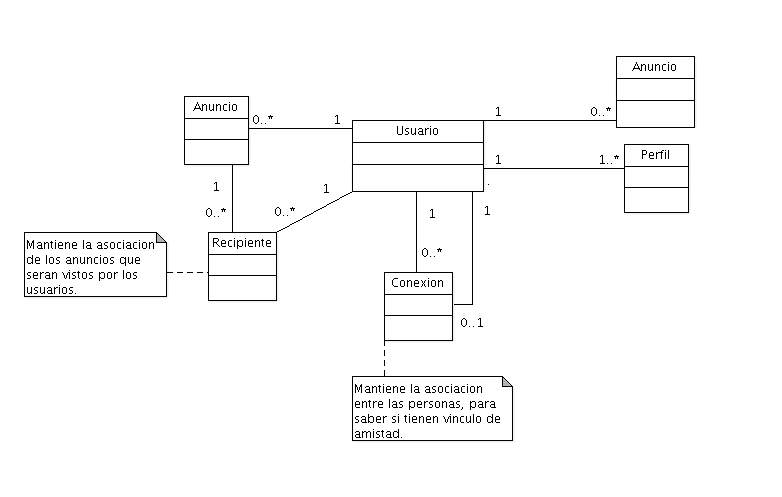
\includegraphics[width=1\textwidth]{file.png}%ext=pdf,jpg,png
\caption{... texto ...}
\label{contexto:figura}
\end{figure}
%\end{document}
